\chapter{FISTA-Net}\label{ch:fistanet}

\section{The paper}

Xiang, Dong and Yang, ``FISTA-Net: Learning a Fast Iterative Shrinkage Thresholding Network for Inverse
Problems in Imaging'', \emph{IEEE Transactions on Medical Imaging}, arXiv 2008.02683. It was tested on
electromagnetic tomography and sparse-view CT.

You chose this because its setup matches ours: a known forward operator $A$, and an unknown image. Your
instruction was to implement the paper as it is, add nothing, and ask whenever unsure.

\begin{keyidea}[The big difference from CSC-LISTA]
CSC-LISTA has no pictures inside: its state is 32 code maps, and it needs a dictionary. FISTA-Net works
directly on the image, needs no dictionary, and replaces the shrink step with a small CNN. It has only 74,599
parameters, against 24.6 million for 32 CSC-LISTA layers. And the same CNN is reused in every layer.
\end{keyidea}

\section{The architecture}

FISTA-Net unrolls FISTA into three modules per stage:
\begin{align}
r^{(k)} &= y^{(k)} - \big(W^{(k)}\big)^T\big(Ay^{(k)} - b\big), \tag{Eq.~8a}\\
x^{(k)} &= \mathcal{T}_{\theta^{(k)}}\big(r^{(k)}\big), \tag{Eq.~8b}\\
y^{(k+1)} &= x^{(k)} + \rho^{(k)}\big(x^{(k)} - x^{(k-1)}\big). \tag{Eq.~8c}
\end{align}

\begin{enumerate}
\item \textbf{Gradient module.} Move the image to better match the measurement. This is where physics enters.
\item \textbf{Proximal module.} A small CNN removes artifacts.
\item \textbf{Momentum module.} FISTA's extrapolation, with a learned weight.
\end{enumerate}

\begin{figure}[H]
\centering
\begin{tikzpicture}[node distance=7mm and 8mm]
\node[fixed] (b) {$b$};
\node[block,right=of b] (init) {Start\\ Eq.~16};
\node[fixed,right=of init] (grad) {Gradient\\ step with $h$,\\ scaled by $\mu^{(k)}$};
\node[learned,right=of grad] (prox) {CNN block\\ threshold $\theta^{(k)}$};
\node[block,right=of prox] (mom) {Momentum\\ $\rho^{(k)}$};
\node[fixed,right=of mom] (out) {$x^{(7)}$};
\draw[flow] (b)--(init); \draw[flow] (init)--(grad); \draw[flow] (grad)--(prox); \draw[flow] (prox)--(mom);
\draw[flow] (mom)--(out);
\draw[flow] (mom.south) -- ++(0,-7mm) -| node[pos=.25,below,note]{repeat for 7 stages, reusing the same CNN} (grad.south);
\end{tikzpicture}
\caption{FISTA-Net. Orange is the shared CNN. $\mu$, $\theta$ and $\rho$ follow learned schedules.}
\end{figure}

\section{Step 1: the starting image, Eq.~16}

\begin{equation}
x^{(0)} = \big(A^TA + \lambda_0 L^TL\big)^{-1} A^T b, \qquad \lambda_0 = 0.001. \tag{Eq.~16}
\end{equation}
$L$ is a matrix of differences between neighbouring pixels. This is a close cousin of Wiener: replace
$\lambda_0L^TL$ with $\mu$ and you get our Wiener filter exactly. Both $A$ and $L$ are convolutions, so each
becomes a simple function of frequency, and the matrix inverse becomes a division.

\begin{code*}{fista_net.py}
def difference_power(n, dtype, device):
    """Fourier symbol of L^T L, with L the row and column differences."""
    fy = torch.fft.fftfreq(n, dtype=dtype, device=device)[:, None]
    fx = torch.fft.rfftfreq(n, dtype=dtype, device=device)[None, :]
    return 4 * (torch.sin(torch.pi * fx) ** 2 + torch.sin(torch.pi * fy) ** 2)
\end{code*}

\begin{code*}{fista_net.py}
    def initial(self, b):
        """Eq. 16: x0 = (A^T A + lambda0 L^T L)^-1 A^T b."""
        n = b.shape[-1]
        h, smooth = self.spectra(n, b)
        return torch.fft.irfft2(torch.fft.rfft2(b) * h / (h * h + smooth), s=(n, n))
\end{code*}

\begin{careful}
The penalty $\lambda_0L^TL$ is very weak at low and middle frequencies, so this start image is far more
aggressive than Wiener. The orange line in Figure~\ref{fig:filters} peaks at a gain of about 80 near a period of
3\um, against Wiener's 2.8. So it starts sharper, and it also amplifies noise much more. The CNN must clean this up.
\end{careful}

\section{Step 2: the gradient module}

This is where the paper and the authors' own code disagree, so this is the first thing I asked you.

\textbf{The paper, Eq.~11--12:} $W^{(k)}=\mu^{(k)}\tilde W$, where $\tilde W$ comes from coherence minimisation.
This is the same weight family as ALISTA.

\textbf{The authors' code, \code{M5FISTANet.py}:}
\begin{equation}
r^{(k)} = y^{(k)} - \mu^{(k)} \big(A^TA + 0.001L^TL\big)^{-1}\big(A^TAy^{(k)} - A^Tb - 0.001L^TLy^{(k)}\big).
\end{equation}

\textbf{You chose the authors' code.} When I asked, I noted that the ALISTA-type weight had amplified noise heavily
on our blur, and that the code's step suits strong blur. Our Fourier form of it:

\begin{code*}{fista_net.py}
    def stage(self, y, b_hat, h, smooth, mu, theta):
        n = y.shape[-1]
        y_hat = torch.fft.rfft2(y)
        step = (h * h * y_hat - h * b_hat - smooth * y_hat) / (h * h + smooth)
        r = y - mu * torch.fft.irfft2(step, s=(n, n))
        return self.block(r, theta)
\end{code*}

\begin{center}
\renewcommand{\arraystretch}{1.4}
\begin{tabular}{ll}
\toprule
Matrix in the code & Fourier form in ours \\
\midrule
$A^TAy$ & \code{h * h * y_hat} \\
$A^Tb$ & \code{h * b_hat} \\
$0.001\,L^TLy$ & \code{smooth * y_hat} \\
$(A^TA + 0.001\,L^TL)^{-1}$ & divide by \code{h * h + smooth} \\
\bottomrule
\end{tabular}
\end{center}

A unit test builds the literal matrices on a small image and confirms that the Fourier version gives the same answer.

\begin{careful}[A sign you should know about]
If you differentiate $\lVert Ay-b\rVert^2+0.001\lVert Ly\rVert^2$, the penalty term comes with a \emph{plus} sign. The authors'
code has a \emph{minus}. Their code comment cites another paper for this formula. Since your instruction was to
follow the authors, we kept the minus, unchanged. I am flagging it so that it does not surprise you. I did not
test the alternative.
\end{careful}

\section{Step 3: the proximal CNN}

\begin{figure}[H]
\centering
\begin{tikzpicture}[node distance=2.5mm,
 c/.style={draw=warm,fill=warmwash,minimum height=11mm,minimum width=6mm,font=\scriptsize,inner sep=1pt},
 t/.style={draw=accent,fill=bluewash,minimum height=11mm,minimum width=9mm,font=\scriptsize,align=center,inner sep=1pt}]
\node[fixed] (in) {$r$};
\node[c,right=of in,xshift=2mm] (d) {$D$};
\node[c,right=of d] (f1) {F1};
\node[c,right=of f1] (f2) {F2};
\node[c,right=of f2] (f3) {F3};
\node[c,right=of f3] (f4) {F4};
\node[t,right=of f4] (st) {soft\\ $\theta^{(k)}$};
\node[c,right=of st] (b1) {B1};
\node[c,right=of b1] (b2) {B2};
\node[c,right=of b2] (b3) {B3};
\node[c,right=of b3] (b4) {B4};
\node[c,right=of b4] (g) {$G$};
\node[circle,draw=ink,inner sep=1pt,right=of g,font=\small] (plus) {$+$};
\node[fixed,right=of plus] (out) {$x$};
\foreach \p/\q in {in/d,d/f1,f1/f2,f2/f3,f3/f4,f4/st,st/b1,b1/b2,b2/b3,b3/b4,b4/g,g/plus,plus/out} \draw[flow] (\p)--(\q);
\draw[flow] (in.north) -- ++(0,9mm) -| (plus.north);
\node[note,above=9mm of st] {skip connection};
\end{tikzpicture}
\caption{The proximal block. Each orange box is a $3\times3$ convolution with 32 channels. ReLU follows F1--F3 and B1--B3.}
\end{figure}

The paper's text describes 8 convolution layers without bias. But the paper also reports 74,599 parameters, and only the
authors' 10-layer block with bias gives that number:
\begin{equation}
\underbrace{320}_{D:\,1\to32} + \underbrace{8\times9{,}248}_{F,\,B:\,32\to32} + \underbrace{289}_{G:\,32\to1}
+ \underbrace{6}_{w_i,\,c_i} = 74{,}599.
\end{equation}
So you chose the code's 10 layers.

\begin{code*}{fista_net.py}
    def forward(self, r, theta):
        start = self.conv_d(r[:, None])
        coded = self.transform(start)
        kept = torch.sign(coded) * F.relu(torch.abs(coded) - theta)
        output = r + self.conv_g(self.inverse(kept))[:, 0]
        symmetry = ((self.inverse(coded) - start) ** 2).mean()
        return output, symmetry, coded.abs().mean()
\end{code*}

This has the same soft-threshold as everywhere else in this booklet, but it acts on a \emph{learned feature space}, $F$,
not on pixels. $\tilde F$ then maps back. The block has a skip connection, so it learns only a correction to $r$.

\section{Step 4: the learned schedules, Eq.~15}

The paper does not let $\mu$, $\theta$ and $\rho$ float freely. Each follows a formula with two learned numbers, so that it
stays positive and changes smoothly with layer $k$:
\begin{align}
\mu^{(k)} &= \mathrm{sp}(w_1k+c_1), \tag{15a}\\
\theta^{(k)} &= \mathrm{sp}(w_2k+c_2), \tag{15b}\\
\rho^{(k)} &= \frac{\mathrm{sp}(w_3k+c_3)-\mathrm{sp}(w_3+c_3)}{\mathrm{sp}(w_3k+c_3)}, \tag{15c}
\end{align}
where $\mathrm{sp}(x)=\ln(1+e^x)$ is the softplus function. The start values are
$\{w_1,w_2,w_3,c_1,c_2,c_3\}=\{-0.5,-0.2,1,-2,-1,0\}$. Run 1 used these. Run 2 used the authors' code values, as explained
at the end of this chapter.

\begin{code*}{fista_net.py}
    def schedules(self, k):
        """Eq. 15 for iteration k, counted from 1."""
        mu = F.softplus(self.w1 * k + self.c1)
        theta = F.softplus(self.w2 * k + self.c2)
        top = F.softplus(self.w3 * k + self.c3)
        return mu, theta, (top - F.softplus(self.w3 + self.c3)) / top
\end{code*}

\begin{figure}[H]
\centering
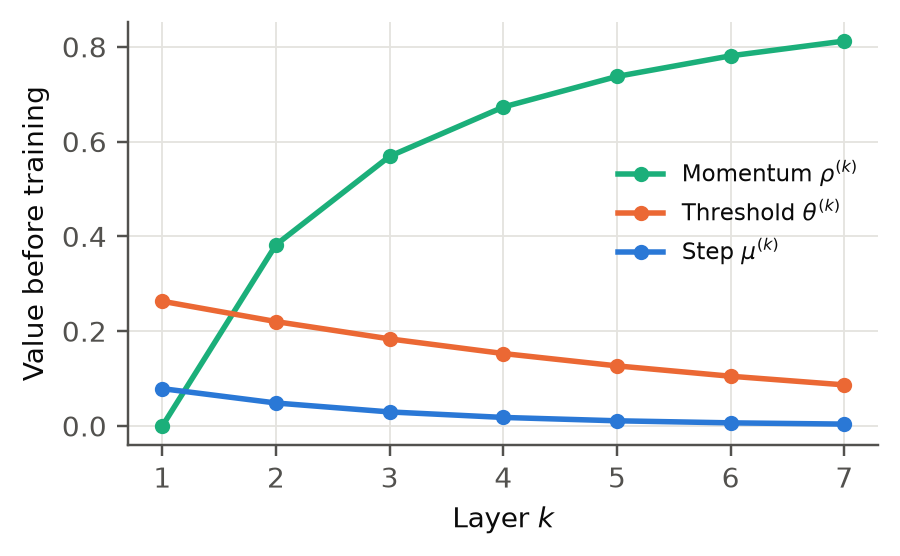
\includegraphics[width=.55\textwidth]{schedules}
\caption{Eq.~15 at the paper's start values, before training.}
\end{figure}

As in FISTA, $\rho$ grows from 0 toward 1. The step and threshold shrink as the image improves. At $k=1$, $\rho=0$
exactly, so the first stage has no momentum.

\section{Step 5: the loss, Eq.~14}

\begin{equation}
L_{\text{total}} = L_{\text{mse}} + \lambda_1 L_{\text{sym}} + \lambda_2 L_{\text{spa}},
\qquad \lambda_1=0.01,\ \lambda_2=0.001 . \tag{Eq.~14}
\end{equation}

\begin{code*}{fista_net.py}
def total_loss(output, target, symmetry, sparsity):
    """Eq. 14 with lambda1 = 0.01 and lambda2 = 0.001."""
    return ((output - target) ** 2).mean() + .01 * symmetry + .001 * sparsity
\end{code*}

\begin{itemize}
\item $L_{\text{mse}}$ compares the final image with the target.
\item $L_{\text{sym}}$ asks $\tilde F$ to undo $F$, so the backward path is a true inverse.
\item $L_{\text{spa}}$ asks the features $F(r)$ to be sparse.
\end{itemize}

\section{The full forward pass}

\begin{code*}{fista_net.py}
    def forward(self, b):
        """b is [B, N, N], zero-padded. Returns field, symmetry and sparsity losses."""
        h, smooth = self.spectra(b.shape[-1], b)
        b_hat = torch.fft.rfft2(b)
        old = y = self.initial(b)
        symmetry = sparsity = 0
        for k in range(1, self.layers + 1):
            mu, theta, rho = self.schedules(k)
            if self.use_checkpoint and self.training:
                x, sym, spa = checkpoint(self.stage, y, b_hat, h, smooth, mu, theta,
                                         use_reentrant=False)
            else:
                x, sym, spa = self.stage(y, b_hat, h, smooth, mu, theta)
            y = x + rho * (x - old)
            old = x
            symmetry, sparsity = symmetry + sym, sparsity + spa
        return x, symmetry, sparsity
\end{code*}

\begin{center}
\renewcommand{\arraystretch}{1.4}
\begin{tabular}{p{6.5cm}p{8cm}}
\toprule
Paper & Code \\
\midrule
$x^{(0)}$, Eq.~16, and $y^{(1)}=x^{(0)}$ & \code{old = y = self.initial(b)} \\
Eq.~15, $k=1\dots N_s$ & \code{self.schedules(k)} \\
Eq.~8a and 8b & \code{self.stage(...)} \\
Eq.~8c & \code{y = x + rho * (x - old)} \\
$\sum_k$ in Eq.~13 & \code{symmetry + sym}, \code{sparsity + spa} \\
Output $x^{(N_s)}$ & \code{return x} \\
\bottomrule
\end{tabular}
\end{center}

\section{Every decision and difference}

\subsection*{Choices you made, when I asked}

\begin{center}
\renewcommand{\arraystretch}{1.3}
\begin{tabularx}{\textwidth}{>{\raggedright\arraybackslash}p{2.8cm}>{\raggedright\arraybackslash}X>{\raggedright\arraybackslash}X>{\raggedright\arraybackslash}p{2.7cm}}
\toprule
Question & Paper & Authors' code & You chose \\
\midrule
Gradient step & $\mu\tilde W$, Eq.~11--12 & Inverse form above & Code \\
CNN & 8 layers, no bias & 10 layers, bias & Code \\
Loss & Eq.~14 & Eq.~14 plus $0.1L_1$ and weight decay & Paper \\
Start values & $\{-0.5,-0.2,1,-2,-1,0\}$ & Different numbers & Paper in run 1, code in run 2 \\
Learning rate & Not given & $10^{-3}$ & Code, without its decay \\
Epochs & Not given & 30 loaded by default & Code \\
\bottomrule
\end{tabularx}
\end{center}

\subsection*{Differences forced by our problem}

\begin{center}
\renewcommand{\arraystretch}{1.3}
\begin{tabularx}{\textwidth}{>{\raggedright\arraybackslash}p{3.3cm}>{\raggedright\arraybackslash}X>{\raggedright\arraybackslash}X}
\toprule
Item & Paper or code & Ours, and why \\
\midrule
Final ReLU & The code forces output $\ge0$ & \textbf{Removed.} Magnetic fields are signed, so it would destroy half the data. This is a real change, and I did not ask you first \\
$A$ and $L$ & Explicit matrices & FFT filters on a padded canvas, because a matrix at this size cannot exist \\
Image size & $64\times64$ EMT images in the paper's first study & 512 pixel crops \\
Batch & 64 & 24, the largest that fits safely \\
Padding & None & 128 pixels of zeros. There is no window mask here, so the gradient step treats the padded zeros as real data \\
\bottomrule
\end{tabularx}
\end{center}

\subsection*{Smaller details that follow the code, not the printed equation}

\begin{center}
\renewcommand{\arraystretch}{1.3}
\begin{tabularx}{\textwidth}{>{\raggedright\arraybackslash}p{3.3cm}>{\raggedright\arraybackslash}X>{\raggedright\arraybackslash}X}
\toprule
Item & Printed Eq.~13 & Ours, following the code \\
\midrule
Symmetry loss & Compares $\tilde F(F(r))$ with $r$ & Compares with the output of \code{conv_D}, $D(r)$, using a mean \\
Sparsity loss & Sum of $\ell_1$ norms & Mean absolute value per layer, summed over layers \\
Layer index & $k=1\dots N_s$ & Same as the paper. The authors' code counts from 0 \\
\bottomrule
\end{tabularx}
\end{center}

\begin{defend}
\textbf{``Did you implement FISTA-Net exactly?''} Say: ``Where the paper and the authors' code disagree, I chose and
recorded which to follow. Two changes are ours: the final ReLU is removed because fields are signed, and the operators
are FFT filters.'' Then point to these tables.
\end{defend}

\section{Training and status}

For run 1: Adam at $10^{-3}$ for everything, no decay, 7 stages, 512 pixel crops, batch 24, 30 epochs. An epoch here means 600 crops,
one per training image, so the run has 750 steps. Validation runs every 25 steps, on the same 64 crops as CSC-LISTA. The
final score uses the same 15 COMSOL pairs. Eight unit tests pass, including the parameter count, Eq.~15, Eq.~16 and the
matrix-versus-Fourier check.

\begin{careful}
Each block of ten $3\times3$ layers sees only 2.1\um\ at 0.1\um\ per pixel, and our wires are about 2\um\ wide. In the paper's
$64\times64$ images, the same block covers a third of the image. The 7 stages together reach 14.1\um, and the gradient
step is global, so this is not a fatal problem. It is simply untested, and it is one thing to look at if the result is poor.
\end{careful}

\section{Run 1: what happened}

\begin{center}
\begin{tabular}{lccc}
\toprule
 & Simulated validation & COMSOL & NRMSE \\
\midrule
Wiener & 60.3\% & 49.3\% & 3.53\% \\
\textbf{FISTA-Net, step 725} & \textbf{65.2\%} & \textbf{39.4\%} & \textbf{2.85\%} \\
Strict Eq.~20, 64 layers & 48.8\% & 33.8\% & 2.43\% \\
\bottomrule
\end{tabular}
\end{center}

The run took 8,332 seconds and peaked at 36.5 GiB. Its 39.4\% was not FISTA-Net's limit, because this run had not
converged.

\begin{figure}[H]
\centering
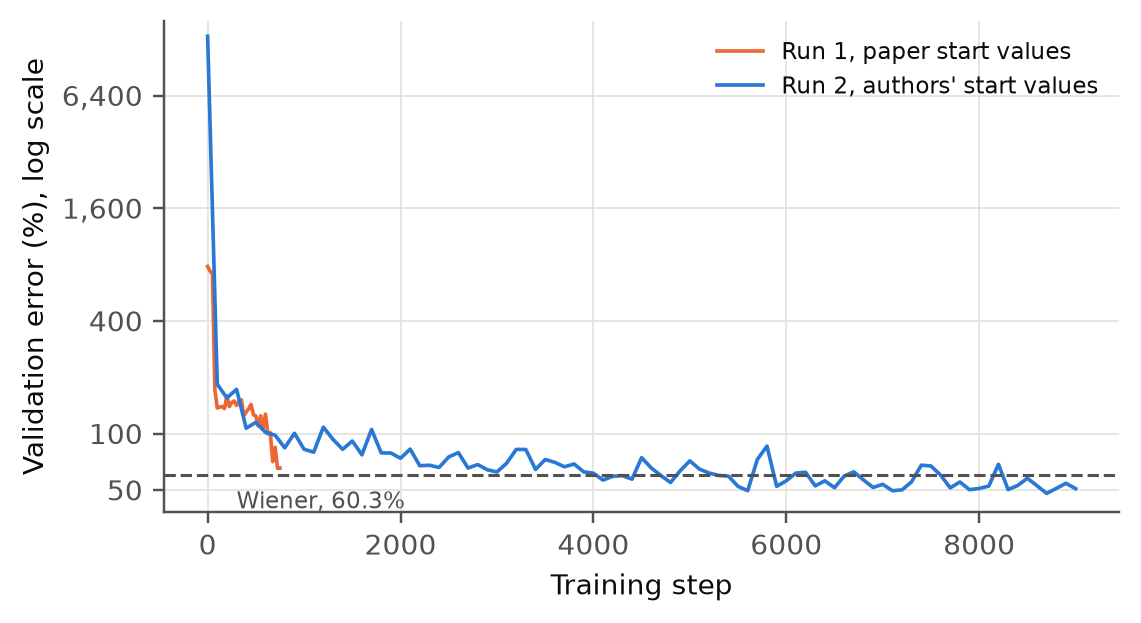
\includegraphics[width=.68\textwidth]{fistanet_curve}
\caption{FISTA-Net validation error during training, for both runs. Run 1 stops at step 750 with no sign of settling.
Run 2 starts far higher and keeps improving for much longer, but it is still noisy at the end.}
\label{fig:fistanet-curve}
\end{figure}

\subsection*{Why the error starts so high}

Before training, the error is 782\%. That comes from the Eq.~16 start image, whose gain of about 80 amplifies the
input noise. A crop with weak signal then gets a huge relative error, and such crops can dominate the mean. This is probably
also why the validation score looks so much worse than the COMSOL score, but I did not test that.

\subsection*{Why I think it stopped short}

\begin{enumerate}
\item \textbf{Far fewer updates.} We trained for 30 epochs of 600 crops at batch 24, which is 750 updates. On the
paper's EMT dataset, 30 epochs at batch 64 would be about 9,000 updates. So ``30 epochs'' was 12 times shorter here.
\item \textbf{The schedules did not learn.} The six scalars barely moved. For example, $w_1$ went from $-0.5$ to $-0.503$, and
$\mu$, $\theta$ and $\rho$ at the last layer stayed at about 0.004, 0.089 and 0.81, so they are effectively still at their
start values.
\item \textbf{The physics step is very small.} See the next section.
\end{enumerate}

\subsection*{A mismatch you should know about}

\begin{careful}[Our start values pair the paper's numbers with the code's gradient step]
You chose the authors' gradient step, and the paper's start values. When I asked, I did not point out how much those
start values differ from the ones in the authors' code, and I should have.
\end{careful}

The authors' code starts $\mu$ at $\mathrm{sp}(0.1-0.2i)$, for $i=0\dots6$. The paper's values give $\mathrm{sp}(-2-0.5k)$.

\begin{center}
\begin{tabular}{lrrrrrrrr}
\toprule
Layer & 1 & 2 & 3 & 4 & 5 & 6 & 7 & Sum \\
\midrule
$\mu$, ours (paper) & 0.079 & 0.049 & 0.030 & 0.018 & 0.011 & 0.007 & 0.004 & 0.197 \\
$\mu$, authors' code & 0.744 & 0.644 & 0.554 & 0.474 & 0.403 & 0.341 & 0.287 & 3.449 \\
\midrule
$\theta$, ours (paper) & 0.263 & 0.220 & 0.184 & 0.153 & 0.127 & 0.105 & 0.087 & \\
$\theta$, authors' code & 0.127 & 0.079 & 0.049 & 0.030 & 0.018 & 0.011 & 0.007 & \\
\bottomrule
\end{tabular}
\end{center}

Summed over the seven stages, our gradient step is about 17 times weaker than in the authors' code, and it never got
larger, because the schedules barely trained. With this inverse-based step, $\mu=1$ would be close to a full jump. Ours adds up to
0.197. So the physics module likely does very little, and the network is mostly a CNN cleaning up the Eq.~16 start image. Our
threshold also starts larger than the code's.

Notice that the paper's $\mu$ numbers, $(-0.5,-2)$, are the numbers the code uses for $\theta$. The paper and the
code may simply have these two labels swapped. I cannot confirm that from the sources.

So run 1 was a fair report of what we ran, but not a fair test of FISTA-Net.

\section{Run 2: the authors' start values and 9,000 updates}

You asked for a rerun. The start values and the length changed, and validation ran less often to keep the cost down.

\begin{center}
\begin{tabular}{lll}
\toprule
 & Run 1 & Run 2 \\
\midrule
Start values & Paper & Authors' code \\
Updates & 750 (30 epochs) & 9,000 (360 epochs) \\
Validation & Every 25 steps & Every 100 steps \\
\bottomrule
\end{tabular}
\end{center}

The code's schedules count from $i=0$ and ours from $k=1$, so the authors' values were rewritten with $c=b-w$. The formula in
Eq.~15 did not change, and a unit test confirms that all seven layers reproduce the authors' $\mu$, $\theta$ and $\rho$.

\begin{code*}{fista_net.py}
START = dict(paper=dict(w1=-.5, w2=-.2, w3=1., c1=-2., c2=-1., c3=0.),
             code=dict(w1=-.2, w2=-.5, w3=.5, c1=.3, c2=-1.5, c3=-.5))
\end{code*}

Everything else stayed the same: the Eq.~14 loss, batch 24, Adam at $10^{-3}$ with no decay, and no final ReLU.

\begin{center}
\begin{tabular}{lccc}
\toprule
 & Simulated validation & COMSOL & NRMSE \\
\midrule
FISTA-Net run 1 & 65.2\% & 39.4\% & 2.85\% \\
FISTA-Net run 2, step 4,800 (interim) & 54.8\% & 34.6\% & 2.50\% \\
\textbf{FISTA-Net run 2, step 8,700} & \textbf{47.9\%} & \textbf{33.3\%} & \textbf{2.41\%} \\
Strict Eq.~20, 64 layers & 48.8\% & 33.8\% & 2.43\% \\
FISTA-300, $\lambda=0.009$ & 35.5\% & 30.5\% & 2.20\% \\
\bottomrule
\end{tabular}
\end{center}

The run took 98,280 seconds, about 27 hours, and also peaked at 36.5 GiB. Fixing the two problems cut the COMSOL error by 6.1
points, and made FISTA-Net the best trained network here, with the fewest parameters.

\subsection*{Reading run 2 honestly}

\begin{itemize}
\item \textbf{It starts much worse.} The first validation error was 13,266\%, against 782\% in run 1. Strong steps
at the start of training amplify the noisy start image further. Training brought this under 115\% by step 500.
\item \textbf{It is still noisy.} In the last 1,000 steps, validation moved between 47.9\% and 68.5\%. The learning rate
never decays, so this may not settle. The best step, 8,700, is partly a lucky draw.
\item \textbf{The schedules still moved little.} At the best step, $\mu$ adds up to 3.166 against the 3.449 it started
from. Most of the learning was in the CNN.
\item \textbf{$B_z$ is its weak spot.} $B_x$ and $B_y$ are at 30.2\% and 30.7\%, better than strict 64 layers, but $B_z$ is at
39.1\%, which is worse. Its worst coil is IC\_4um, at 34.6\%.
\item \textbf{It is not at a limit yet.} Validation was still improving late in the run, so we do not know where it would stop.
\end{itemize}

\begin{keyidea}[What this means]
Our first low score came from our own setup, not from the method. Run 2 is a fair test, and it puts FISTA-Net level with
the much larger CSC-LISTA. It still does not reach FISTA-300's 30.5\%.
\end{keyidea}

The output on the COMSOL crop is in Figure~\ref{fig:reconstruction-new}.
